% Options for packages loaded elsewhere
\PassOptionsToPackage{unicode}{hyperref}
\PassOptionsToPackage{hyphens}{url}
%
\documentclass[
]{book}
\usepackage{amsmath,amssymb}
\usepackage{iftex}
\ifPDFTeX
  \usepackage[T1]{fontenc}
  \usepackage[utf8]{inputenc}
  \usepackage{textcomp} % provide euro and other symbols
\else % if luatex or xetex
  \usepackage{unicode-math} % this also loads fontspec
  \defaultfontfeatures{Scale=MatchLowercase}
  \defaultfontfeatures[\rmfamily]{Ligatures=TeX,Scale=1}
\fi
\usepackage{lmodern}
\ifPDFTeX\else
  % xetex/luatex font selection
\fi
% Use upquote if available, for straight quotes in verbatim environments
\IfFileExists{upquote.sty}{\usepackage{upquote}}{}
\IfFileExists{microtype.sty}{% use microtype if available
  \usepackage[]{microtype}
  \UseMicrotypeSet[protrusion]{basicmath} % disable protrusion for tt fonts
}{}
\makeatletter
\@ifundefined{KOMAClassName}{% if non-KOMA class
  \IfFileExists{parskip.sty}{%
    \usepackage{parskip}
  }{% else
    \setlength{\parindent}{0pt}
    \setlength{\parskip}{6pt plus 2pt minus 1pt}}
}{% if KOMA class
  \KOMAoptions{parskip=half}}
\makeatother
\usepackage{xcolor}
\usepackage{color}
\usepackage{fancyvrb}
\newcommand{\VerbBar}{|}
\newcommand{\VERB}{\Verb[commandchars=\\\{\}]}
\DefineVerbatimEnvironment{Highlighting}{Verbatim}{commandchars=\\\{\}}
% Add ',fontsize=\small' for more characters per line
\usepackage{framed}
\definecolor{shadecolor}{RGB}{248,248,248}
\newenvironment{Shaded}{\begin{snugshade}}{\end{snugshade}}
\newcommand{\AlertTok}[1]{\textcolor[rgb]{0.94,0.16,0.16}{#1}}
\newcommand{\AnnotationTok}[1]{\textcolor[rgb]{0.56,0.35,0.01}{\textbf{\textit{#1}}}}
\newcommand{\AttributeTok}[1]{\textcolor[rgb]{0.13,0.29,0.53}{#1}}
\newcommand{\BaseNTok}[1]{\textcolor[rgb]{0.00,0.00,0.81}{#1}}
\newcommand{\BuiltInTok}[1]{#1}
\newcommand{\CharTok}[1]{\textcolor[rgb]{0.31,0.60,0.02}{#1}}
\newcommand{\CommentTok}[1]{\textcolor[rgb]{0.56,0.35,0.01}{\textit{#1}}}
\newcommand{\CommentVarTok}[1]{\textcolor[rgb]{0.56,0.35,0.01}{\textbf{\textit{#1}}}}
\newcommand{\ConstantTok}[1]{\textcolor[rgb]{0.56,0.35,0.01}{#1}}
\newcommand{\ControlFlowTok}[1]{\textcolor[rgb]{0.13,0.29,0.53}{\textbf{#1}}}
\newcommand{\DataTypeTok}[1]{\textcolor[rgb]{0.13,0.29,0.53}{#1}}
\newcommand{\DecValTok}[1]{\textcolor[rgb]{0.00,0.00,0.81}{#1}}
\newcommand{\DocumentationTok}[1]{\textcolor[rgb]{0.56,0.35,0.01}{\textbf{\textit{#1}}}}
\newcommand{\ErrorTok}[1]{\textcolor[rgb]{0.64,0.00,0.00}{\textbf{#1}}}
\newcommand{\ExtensionTok}[1]{#1}
\newcommand{\FloatTok}[1]{\textcolor[rgb]{0.00,0.00,0.81}{#1}}
\newcommand{\FunctionTok}[1]{\textcolor[rgb]{0.13,0.29,0.53}{\textbf{#1}}}
\newcommand{\ImportTok}[1]{#1}
\newcommand{\InformationTok}[1]{\textcolor[rgb]{0.56,0.35,0.01}{\textbf{\textit{#1}}}}
\newcommand{\KeywordTok}[1]{\textcolor[rgb]{0.13,0.29,0.53}{\textbf{#1}}}
\newcommand{\NormalTok}[1]{#1}
\newcommand{\OperatorTok}[1]{\textcolor[rgb]{0.81,0.36,0.00}{\textbf{#1}}}
\newcommand{\OtherTok}[1]{\textcolor[rgb]{0.56,0.35,0.01}{#1}}
\newcommand{\PreprocessorTok}[1]{\textcolor[rgb]{0.56,0.35,0.01}{\textit{#1}}}
\newcommand{\RegionMarkerTok}[1]{#1}
\newcommand{\SpecialCharTok}[1]{\textcolor[rgb]{0.81,0.36,0.00}{\textbf{#1}}}
\newcommand{\SpecialStringTok}[1]{\textcolor[rgb]{0.31,0.60,0.02}{#1}}
\newcommand{\StringTok}[1]{\textcolor[rgb]{0.31,0.60,0.02}{#1}}
\newcommand{\VariableTok}[1]{\textcolor[rgb]{0.00,0.00,0.00}{#1}}
\newcommand{\VerbatimStringTok}[1]{\textcolor[rgb]{0.31,0.60,0.02}{#1}}
\newcommand{\WarningTok}[1]{\textcolor[rgb]{0.56,0.35,0.01}{\textbf{\textit{#1}}}}
\usepackage{longtable,booktabs,array}
\usepackage{calc} % for calculating minipage widths
% Correct order of tables after \paragraph or \subparagraph
\usepackage{etoolbox}
\makeatletter
\patchcmd\longtable{\par}{\if@noskipsec\mbox{}\fi\par}{}{}
\makeatother
% Allow footnotes in longtable head/foot
\IfFileExists{footnotehyper.sty}{\usepackage{footnotehyper}}{\usepackage{footnote}}
\makesavenoteenv{longtable}
\usepackage{graphicx}
\makeatletter
\def\maxwidth{\ifdim\Gin@nat@width>\linewidth\linewidth\else\Gin@nat@width\fi}
\def\maxheight{\ifdim\Gin@nat@height>\textheight\textheight\else\Gin@nat@height\fi}
\makeatother
% Scale images if necessary, so that they will not overflow the page
% margins by default, and it is still possible to overwrite the defaults
% using explicit options in \includegraphics[width, height, ...]{}
\setkeys{Gin}{width=\maxwidth,height=\maxheight,keepaspectratio}
% Set default figure placement to htbp
\makeatletter
\def\fps@figure{htbp}
\makeatother
\setlength{\emergencystretch}{3em} % prevent overfull lines
\providecommand{\tightlist}{%
  \setlength{\itemsep}{0pt}\setlength{\parskip}{0pt}}
\setcounter{secnumdepth}{5}
\usepackage{booktabs}
\ifLuaTeX
  \usepackage{selnolig}  % disable illegal ligatures
\fi
\usepackage[]{natbib}
\bibliographystyle{plainnat}
\IfFileExists{bookmark.sty}{\usepackage{bookmark}}{\usepackage{hyperref}}
\IfFileExists{xurl.sty}{\usepackage{xurl}}{} % add URL line breaks if available
\urlstyle{same}
\hypersetup{
  pdftitle={Comandos básicos do R: Guia de bolso},
  pdfauthor={Lucas C. Germano},
  hidelinks,
  pdfcreator={LaTeX via pandoc}}

\title{Comandos básicos do R: Guia de bolso}
\author{Lucas C. Germano}
\date{Tue Jul 11 08:20:32 2023}

\usepackage{amsthm}
\newtheorem{theorem}{Theorem}[chapter]
\newtheorem{lemma}{Lemma}[chapter]
\newtheorem{corollary}{Corollary}[chapter]
\newtheorem{proposition}{Proposition}[chapter]
\newtheorem{conjecture}{Conjecture}[chapter]
\theoremstyle{definition}
\newtheorem{definition}{Definition}[chapter]
\theoremstyle{definition}
\newtheorem{example}{Example}[chapter]
\theoremstyle{definition}
\newtheorem{exercise}{Exercise}[chapter]
\theoremstyle{definition}
\newtheorem{hypothesis}{Hypothesis}[chapter]
\theoremstyle{remark}
\newtheorem*{remark}{Remark}
\newtheorem*{solution}{Solution}
\begin{document}
\maketitle

{
\setcounter{tocdepth}{1}
\tableofcontents
}
\hypertarget{sobre-este-livro}{%
\chapter*{Sobre este livro}\label{sobre-este-livro}}
\addcontentsline{toc}{chapter}{Sobre este livro}

Sejam bem-vindos!\\
O objetivo deste livro é disponibilizar para consulta anotações de códigos R de forma prática e rápida. Não há explicações aprofundadas nem se pretende esgotar as possibilidades do conteúdo apresentado, assim, esta documentação deve ser utilizada somente como um guia rápido, pois não passa de um conjunto de rascunhos apreendidos no dia-a-dia da manipulação de dados e na apresentação de resultados. O conteúdo poderá ser baixado nos formatos \texttt{.pdf} ou \texttt{epub}, mas a proposta é que o conteúdo seja dinâmico, com atualizações frequentes. Toda estrutura deste e-book encontra-se disponível no \href{https://github.com/lucascgmermano/guia_de_bolso.git}{GitHub}.\\
Críticas, sugestões ou contribuições de código e conteúdo podem ser enviadas para \url{lucascgermano@gmail.com}, ficarei muito feliz, qualquer que seja o motivo do contato.

\hypertarget{leitura-e-escrita-de-arquivos-de-texto}{%
\chapter{Leitura e escrita de arquivos de texto}\label{leitura-e-escrita-de-arquivos-de-texto}}

\hypertarget{diretuxf3rio-de-trabalho}{%
\section{Diretório de trabalho}\label{diretuxf3rio-de-trabalho}}

Abaixo são transcritos alguns comandos e métodos para se definir e conhecer o diretório de trabalho, criar e excluir pastas e arquivos.

\begin{longtable}[]{@{}
  >{\raggedright\arraybackslash}p{(\columnwidth - 2\tabcolsep) * \real{0.4444}}
  >{\raggedright\arraybackslash}p{(\columnwidth - 2\tabcolsep) * \real{0.5556}}@{}}
\caption{Comandos de definição e manipulação de diretórios e arquivos.}\tabularnewline
\toprule\noalign{}
\begin{minipage}[b]{\linewidth}\raggedright
Comando
\end{minipage} & \begin{minipage}[b]{\linewidth}\raggedright
Definição
\end{minipage} \\
\midrule\noalign{}
\endfirsthead
\toprule\noalign{}
\begin{minipage}[b]{\linewidth}\raggedright
Comando
\end{minipage} & \begin{minipage}[b]{\linewidth}\raggedright
Definição
\end{minipage} \\
\midrule\noalign{}
\endhead
\bottomrule\noalign{}
\endlastfoot
base::setwd() & Define diretório de trabalho. \\
base::getwd() & Identifica diretório ativo. \\
base::dir() & Retorna todo o conteúdo do diretório ativo. \\
Ctrl + Shift + h & Abre janela de navegação para definir diretório. \\
base::file.choose() & Abre janela de navegação e ao selecionar o arquivo, ele retorna o caminho (diretório). Pode-se usar também dentro do comando, como em read.csv2(file = file.choose()). \\
No RStudio: Ir em Session, Setting Working Directory & Equivalente a Ctrl + Shift + h \\
Inserir aspas ' ' + Tab entre elas & Navegação que pode servir para explorar caminhos. \\
base::dir.create() & Cria uma pasta de trabalho. \\
base::unlink() & Deleta uma pasta, ex. unlink(``some\_directory'', recursive = TRUE). Aceita um vetor c() para excluir vários arquivos ou pastas. \\
base::file.create() & Cria um arquivo no diretório ex. file.create(``text\_file.txt'') (docx, csv, etc). \\
base::file.copy() & Copia um arquivo. Ex. file.copy(from = ``source\_file.txt'', to = ``destination\_folder''). \\
base::file.remove() & Deleta um arquivo, ex. file.remove(``csv\_file.csv''). Pode-se usar também unlink(`csv\_file.csv'). \\
base::file.rename() & Renomear um arquivo. \\
base::list.files() & Lista os arquivos presentes no diretório. \\
here::here() & Cria um caminho relativo para um arquivo no diretório de trabalho, preferencialmente em um projeto, o que facilita ser reproduzido em diversas máquinas, ex. here(`arquivos',`dados.csv'). É similar ao base::file.path(), cuja sintaxe é a mesma. \\
\end{longtable}

\textbf{Exemplo: list.files()}

\begin{verbatim}
list.files(path = 'dados/',      # Caminho do arquivo
           pattern = '.ods',     # Formato especificado
           full.names = FALSE,   # Somente nome
           recursive = TRUE,     # Pesquisa em subpastas
           ignore.case = FALSE)  # Ignora tamanhos das letras
\end{verbatim}

\hypertarget{leitura-de-arquivos}{%
\section{Leitura de arquivos}\label{leitura-de-arquivos}}

\hypertarget{utilsread.csv2}{%
\subsection{utils::read.csv2()}\label{utilsread.csv2}}

Faz a leitura de um arquivo em formado de tabela e cria um data frame a partir dele, com casos como linhas e variáveis como colunas. É uma função nativa do R, em que read.csv trata de arquivos separados por vírgula, enquanto read.csv2 de arquivos separados por ponto e vírgula. Os argumentos das funções são os mesmos, por isso o .csv2 foi escolhido para o exemplo (\href{https://www.rdocumentation.org/packages/utils/versions/3.6.2/topics/read.table}{documentação})

\begin{quote}
\textbf{Exemplo}
\end{quote}

\begin{verbatim}
dados <- read.csv2(file = 'dados/dados.csv')
head(dados, 2)          # Exibir as 2 primeiras linhas dos dados.
\end{verbatim}

\begin{quote}
\textbf{Argumentos principais}
\end{quote}

\begin{longtable}[]{@{}
  >{\raggedright\arraybackslash}p{(\columnwidth - 2\tabcolsep) * \real{0.5000}}
  >{\raggedright\arraybackslash}p{(\columnwidth - 2\tabcolsep) * \real{0.5000}}@{}}
\toprule\noalign{}
\begin{minipage}[b]{\linewidth}\raggedright
Argumento
\end{minipage} & \begin{minipage}[b]{\linewidth}\raggedright
Definição
\end{minipage} \\
\midrule\noalign{}
\endhead
\bottomrule\noalign{}
\endlastfoot
file & Nome do arquivo que será lido, contendo o caminho do diretório. \\
header & Logical. Indica se o arquivo contém os nomes das colunas na primeira linha. \\
sep & Tipo de separador de campo. Default é = ``;''. \\
dec & Tipo de separador de decimal. Default é = ``.''. \\
nrows & Integer. Número máximo de linhas a serem lidas. \\
skip & Integer. Número de linhas que serão puladas antes de iniciar a leitura dos dados. \\
fill & Logical. Se TRUE, caso as linhas tenham comprimento desigual, seão adicionados campos em branco. \\
blank.lines.skip & Logical. Se TRUE linhas vazias serão ignoradas. \\
stringsAsFactors & Logical. Se TRUE os vetores character serão convertidos para factors. Se houver distorção dos caracteres, utilizar FALSE para sem conversão. \\
fileEncoding & Character string. Define o encoding que será usado. Ex. fileEnconding = ``UTF-8'' ou ``Latin-1'' ou ``ISO-8859-1''. \\
skipNull & Logical. Se TRUE os nulos (NA) devem ser ignorados. \\
colClasses & character. Um vetor de classes referentes as colunas. Valores possíveis são NA (default, quando type.convert é usado), ``NULL'' (quando a coluna é pulada), um vetor atomico de classes(logical, integer, numeric, complex, character, raw), or ``factor'', ``Date'' or ``POSIXct''. \\
\end{longtable}

\begin{itemize}
\tightlist
\item
  \emph{Os argumentos são os mesmos da função read.table().}
\end{itemize}

\hypertarget{readrread_csv2}{%
\subsection{readr::read\_csv2()}\label{readrread_csv2}}

O objetivo do readr é fornecer uma maneira rápida e amigável de ler dados retangulares (como csv, tsv e fwf). Ele foi projetado para analisar de forma flexível muitos tipos de dados encontrados. Já está integrado no RStudio no método de importação via interface gráfica, embora necessite de instalação (\href{https://www.rdocumentation.org/packages/readr/versions/1.3.1}{Documentação})

\begin{quote}
\textbf{Exemplo 1}
\end{quote}

\begin{verbatim}
dados <- readr::read_csv2(file = 'dados/dados.csv',  # Caminho e arquivo
                          col_select = c(2,4:7),     # Seleção de colunas
                          guess_max = 1000,          # Máximo de linhas utilizadas para adivinhar classes
                          skip_empty_rows = TRUE)    # Pular linhas vazias
\end{verbatim}

\begin{quote}
\textbf{Exemplo 2}
\end{quote}

\begin{verbatim}
dados <- readr::read_csv2(
              file = 'dados/dados.csv',    # Caminho e arquivo
              guess_max = 1000,            # Linhas utilizadas para classes
              col_types = c(X = "double"), # A primeira coluna será double. Um vetor com tipos de classes.
              skip_empty_rows = TRUE,      # Pular linhas vazias
              skip = 1,                    # Pular primeira linha
              col_names = c('a','b','c','d','e'),   # Definir nomes das colunas
              col_select = c('a','b','c','d','e'))  # Selecionar colunas
\end{verbatim}

\begin{quote}
\textbf{Argumentos principais}
\end{quote}

\begin{longtable}[]{@{}
  >{\raggedright\arraybackslash}p{(\columnwidth - 2\tabcolsep) * \real{0.5000}}
  >{\raggedright\arraybackslash}p{(\columnwidth - 2\tabcolsep) * \real{0.5000}}@{}}
\toprule\noalign{}
\begin{minipage}[b]{\linewidth}\raggedright
Argumento
\end{minipage} & \begin{minipage}[b]{\linewidth}\raggedright
Definição
\end{minipage} \\
\midrule\noalign{}
\endhead
\bottomrule\noalign{}
\endlastfoot
file & Nome do arquivo que será lido, contendo o caminho do diretório (admite http). Arquivos terminados em .gz, .bz2, .xz, ou .zip serão automaticamente descomprimidos. \\
col\_names & TRUE ou FALSE ou um vetor tipo caracter com nomes das colunas. Se TRUE, a primeira linha será usada para nomear as colunas. Se FALSE, nomes das colunas serão gerados automaticamente (X1, X2, X3 etc). Se col\_names for um vetor com nomes, os valores serão usados como nomes das colunas, mas a primeira linha será considerada no banco (nomes errados), assim, pode-se usar o argumento renomeando as colunas, mas fazendo a leitura sem considerar a primeira linha, com {[}-1,{]} ou skip = 1. Colunas sem nome (NA) receberão nomes fictícios. \\
col\_types & Se for NULL, todos as classes de coluna serão imputadas a partir do máximo de linhas lidas (guess\_max) intercaladas por todo o arquivo. Se a imputação falhar, você precisará aumentar o guess\_max ou fornecer os tipos corretos você mesmo. As especificações de coluna criadas por list() ou cols() devem conter uma especificação de coluna para cada coluna. Se você quiser ler apenas um subconjunto das colunas, use cols\_only(). Para compactar um vetor com as classes, usar as letras c = character, i = integer, n = number, d = double, l = logical, f = factor, D = date, T = date time, t = time, ? = guess. Por padrão, a definição de classe é automática. \\
col\_select & Colunas a serem incluídas nos resultados, equivale a dplyr::select() para se referir às colunas pelo nome. Use c() ou list() para usar mais de uma expressão de seleção. Embora esse uso seja menos comum, col\_select também aceita um índice de coluna numérica. \\
locale & A localidade controla os padrões que variam de lugar para lugar. A localidade padrão é centrada nos EUA (como R), mas você pode usar locale() para criar sua própria localidade que controla coisas como o fuso horário padrão, codificação, marca decimal, marca grande e nomes de dia e mês. \\
na & Vetor de caracteres de strings para interpretar como valores ausentes. Defina esta opção como character() para indicar que não há valores ausentes. \\
trim\_ws & Os espaços em branco à esquerda e à direita (espaços e tabulações ASCII) devem ser cortados de cada campo antes de analisá-lo? \\
skip & Número de linhas para pular antes de ler os dados. \\
n\_max & Número máximo de linhas a ler. \\
guess\_max & Número máximo de linhas a serem usadas para adivinhar os tipos de coluna. \\
show\_col\_types & Se FALSE, não mostre os tipos de coluna adivinhados. Se TRUE sempre mostra os tipos de coluna, mesmo que sejam fornecidos. Se NULL (o padrão) mostrar apenas os tipos de coluna se eles não forem fornecidos explicitamente pelo argumento col\_types. \\
skip\_empty\_rows & As linhas em branco devem ser ignoradas completamente? ou seja, se esta opção for TRUE, as linhas em branco não serão representadas. Se for FALSE, eles serão representados por valores NA em todas as colunas. \\
\end{longtable}

\hypertarget{data.tablefread}{%
\subsection{data.table::fread()}\label{data.tablefread}}

Similar ao read.table e read.csv, só que mais rápido e conveniente por ler arquivos muito grandes. Todos os controles como sep, colClasses, nrows, encoding são detectados atuomaticamente. O resultado padrão é um objeto data.table, mas pode-se mudar para data.frame (\href{https://www.rdocumentation.org/packages/data.table/versions/1.14.2/topics/fread}{documentação}).

\begin{quote}
\textbf{Exemplo}
\end{quote}

\begin{verbatim}
dados <- data.table::fread(file = 'dados/dados.csv',            # Caminho do arquivo
                           select = c("data","muni","casos"),   # Seleciona colunas
                           colClasses = c(data = "Date",        # Define classes
                                          muni = "character",
                                          casos = "integer"),
                           col.names = c("data.in.sin",         # Renomeia colunas
                                         "municipio", 
                                         "num_casos")) 
\end{verbatim}

\begin{quote}
\textbf{Argumentos principais}
\end{quote}

\begin{longtable}[]{@{}
  >{\raggedright\arraybackslash}p{(\columnwidth - 2\tabcolsep) * \real{0.5000}}
  >{\raggedright\arraybackslash}p{(\columnwidth - 2\tabcolsep) * \real{0.5000}}@{}}
\toprule\noalign{}
\begin{minipage}[b]{\linewidth}\raggedright
Argumento
\end{minipage} & \begin{minipage}[b]{\linewidth}\raggedright
Definição
\end{minipage} \\
\midrule\noalign{}
\endhead
\bottomrule\noalign{}
\endlastfoot
file & Nome do arquivo no diretório de trabalho, caminho para o arquivo ou um URL começando http:, etc. Arquivos compactados `.gz' e `.bz2' são suportados se o pacote R.utils estiver instalado. \\
sep & O separador entre colunas. \\
nrows & Número máximo de linhas a serem lidas. \\
header & Logical. Primeria linha é o nome das colunas. \\
na.strings & Para ler NA, como NA, defina na.strings=``NA''. Para ler ,, como string em branco ``\,``, defina na.strings=NULL. \\
stringsAsFactors & Converter todas as colunas de caracteres em fatores? \\
skip & skip \textgreater0 ignora as primeiras linhas. skip=``string'' procura por ``string'' no arquivo (por exemplo, uma substring da linha de nomes de coluna) e começa nessa linha (inspirada em read.xls no pacote gdata). \\
select & Um vetor de nomes de colunas ou números para manter e eliminar as demais. Pode especificar também tipos da mesma forma que colClasses; ou seja, um vetor de pares colname=type, ou uma lista de pares type=col(s). Em todas as formas de seleção, a ordem em que as colunas são especificadas determina a ordem das colunas no resultado. \\
drop & Vetor de nomes de colunas ou números a serem descartados, mantenha o resto. \\
colClasses & Pode receber um vetor ou lista nomeado especificando tipos para um subconjunto das colunas por nome. O padrão NULL significa que os tipos são inferidos automaticamente. Ex1 - colClasses = c(``Date'', ``character'',``integer''), neste caso as classes vão compor as classes das colunas na ordem posta. Ex2 - colClasses = c(``data'' = ``Date'', ``idade'' = ``integer''), nesse caso estou indicando as classes somente de algumas variaveis. Funciona também no read.csv2. \\
dec & Separador de decimal como em read.csv2. \\
col.names & Inserir um vetor de nomes para as colunas se quiser substituir os originais. Se houver alguma coluna original sem título (NA), ela será renomeada automaticamente com ``V''+ o numero que corresponde no banco (V1,V2,V3). \\
encoding & Default is ``unknown''. Outras possíveis opções são ``UTF-8'' e ``Latin-1''. Porém, não é usado para recodificar, em vez disso, permite o manuseio de strings codificadas em sua codificação nativa. \\
strip.white & O padrão é TRUE. Retira espaços em branco à esquerda e à direita de campos não citados. Se FALSE, apenas os espaços à direita do cabeçalho serão removidos. \\
fill & Logical, o padrão é FALSE. Se TRUE, caso as linhas tenham comprimento desigual, os campos em branco serão preenchidos implicitamente. \\
blank.lines.skip & Logical, o padrão é FALSE. Se TRUE, as linhas em branco serão ignoradas. \\
showProgress & TRUE exibe o progresso no console se o ETA for maior que 3 segundos. \\
data.table & TRUE retorna um data.table (default). FALSE retorna um data.frame. O default para este argumento pode ser modificado com opcões(datatable.fread.datatable=FALSE). \\
nThread & Número de threads a serem usados. Experimente para ver o que funciona melhor para seus dados em seu hardware. \\
KeepLeadingZeros & Se for TRUE, dados numéricos com zeros à esquerda seão lidos como caracterer, caso contrário, os zeros à esquerda serão removidos e convertidos em numéricos. \\
\end{longtable}

\hypertarget{readodsread_ods}{%
\subsection{readODS::read\_ods()}\label{readodsread_ods}}

Função para leitura de arquivos no formato .ods do Libre Office. A leitura é feita em somente uma planilha, retorna um data.frame e costuma ser um pouco mais lenta comparada aos outros formatos (\href{https://www.rdocumentation.org/packages/readODS/versions/1.7.0/topics/read_ods}{documentação}).

\begin{quote}
\textbf{Exemplo}
\end{quote}

\begin{verbatim}
dados <- readODS::read_ods(path = 'dados/planilha_ods.ods',  # Caminho do arquivo
                           col_names = FALSE,                # Primeira linha contém nomes das colunas
                           sheet = 1,                        # Seleção da planilha
                           range = "A7:B14")                 # Intervalo para leitura
\end{verbatim}

\begin{quote}
\textbf{Argumentos principais}
\end{quote}

\begin{longtable}[]{@{}
  >{\raggedright\arraybackslash}p{(\columnwidth - 2\tabcolsep) * \real{0.5000}}
  >{\raggedright\arraybackslash}p{(\columnwidth - 2\tabcolsep) * \real{0.5000}}@{}}
\toprule\noalign{}
\begin{minipage}[b]{\linewidth}\raggedright
Argumento
\end{minipage} & \begin{minipage}[b]{\linewidth}\raggedright
Definição
\end{minipage} \\
\midrule\noalign{}
\endhead
\bottomrule\noalign{}
\endlastfoot
path & Caminho do arquivo ods. \\
sheet & Planilha que será lida. Default e 1. Pode ser o nome da planilha (ex. ``semana1'') ou um número correspondente a planilha. \\
col\_names & Indica se a primeira linha contem os nomes das colunas. \\
skip & Número de linhas a pular antes de iniciar a leitura dos dados. \\
formula\_as\_formula & Exibir fórmulas como fórmulas ``SUM(A1:A3)'' ou como valores ``3'' ou ``8''. \\
range & Seleção de retângulo usando intervalo de células semelhante ao Excel, como intervalo = ``D12:F15'' ou intervalo = ``R1C12:R6C15''. O processamento de intervalo de células é tratado pelo pacote cellranger. \\
row\_names & Indica se o arquivo contém os nomes das linhas na primeira coluna. \\
strings\_as\_factors & Logical. Se variáveis tipo character serão convertidas a fatores. \\
\end{longtable}

\hypertarget{readxlread_excel}{%
\subsection{readxl::read\_excel()}\label{readxlread_excel}}

Leitura de arquivos com extensão .xls e xlsx, lidos pelo Excel e Libre Office. Por padrão, a sheet 1 é lida se não houver definição (\href{https://www.rdocumentation.org/packages/readxl/versions/0.1.1/topics/read_excel}{documentação}).

\begin{quote}
\textbf{Exemplo}
\end{quote}

\begin{verbatim}
   dados <- readxl::read_excel(path = "dados/planilha_xlsx.xlsx",
                   sheet = 1,                          # seleciona a planilha 1
                   col_names = c('vel','dist'),        # seleciona colunas (não renomeia)
                   col_types = c("numeric","numeric"), # define a classe
                   range = "A3:B19")                   # define intervalo de leitura da planilha
\end{verbatim}

\begin{quote}
\textbf{Argumentos principais}
\end{quote}

\begin{longtable}[]{@{}
  >{\raggedright\arraybackslash}p{(\columnwidth - 2\tabcolsep) * \real{0.5000}}
  >{\raggedright\arraybackslash}p{(\columnwidth - 2\tabcolsep) * \real{0.5000}}@{}}
\toprule\noalign{}
\begin{minipage}[b]{\linewidth}\raggedright
Argumento
\end{minipage} & \begin{minipage}[b]{\linewidth}\raggedright
Definição
\end{minipage} \\
\midrule\noalign{}
\endhead
\bottomrule\noalign{}
\endlastfoot
path & Caminho para o arquivo xls/xlsx. \\
sheet & Planilha a ser lida. Aceita o nome da planilha ou o número correspondente. Default é a primeira planilha. \\
reange & Intervalo de células para leitura, ex. ``B3:D87'' ou ``Orçamento!B2:G14''. \\
col\_names & Se TRUE a primeira linha será usada para nomear as colunas. FALSE o número das colunas será uma sequência automática de X1 a Xn, ou um vetor de nomes para cada coluna. \\
col\_types & Se NULL os tipos de classes serão adivinhados, senão inserir um vetor indicando as classes ``blank'', ``numeric'', ``date'' or ``text''. \\
na & Valores ausentes. Por default o readxl converte celulas em branco para valores ausentes. Pode-se inserir um valor padrão caso se deseje cobrir os valores ausentes. \\
skip & Número de linhas para pular antes de iniciar a leitura dos dados. \\
n\_max & Número máximo de linhas a serem lidas. \\
guess\_max & Máximo de linhas utilizados para adivinhar classes das colunas. \\
\end{longtable}

\hypertarget{foreignread.dbf}{%
\subsection{foreign::read.dbf()}\label{foreignread.dbf}}

A função le arquivos .dbf como dataframe, convertendo por default campos character em factor. Tem apenas dois argumentos, o file (caminho) e o as.is (se FALSE não converte os campos em factor). Por não ser muito usado, o desenvolvedor já alerta que nem todos os arquivos poderão ser lidos normalmente (\href{https://www.rdocumentation.org/packages/foreign/versions/0.8-82/topics/read.dbf}{documentação}).

\begin{quote}
\textbf{Exemplo}
\end{quote}

\begin{verbatim}
dados <- foreign::read.dbf(file = 'dados/planilha_dbf.dbf')
\end{verbatim}

\begin{quote}
\textbf{Argumentos principais}
\end{quote}

\begin{longtable}[]{@{}
  >{\raggedright\arraybackslash}p{(\columnwidth - 2\tabcolsep) * \real{0.5000}}
  >{\raggedright\arraybackslash}p{(\columnwidth - 2\tabcolsep) * \real{0.5000}}@{}}
\toprule\noalign{}
\begin{minipage}[b]{\linewidth}\raggedright
Argumento
\end{minipage} & \begin{minipage}[b]{\linewidth}\raggedright
Definição
\end{minipage} \\
\midrule\noalign{}
\endhead
\bottomrule\noalign{}
\endlastfoot
file & O caminho para o arquivo DBF que você deseja ler. \\
as.is & Um valor lógico indicando se as strings devem ser retornadas como estão (sem conversão para fatores ou caracteres). \\
as.data.frame & Um valor lógico indicando se o resultado deve ser convertido em um objeto de classe data.frame. \\
NA & Um valor para representar valores ausentes no arquivo DBF. \\
encoding & A codificação dos caracteres no arquivo DBF. \\
convert.factors & Um valor lógico indicando se as colunas de fatores devem ser convertidas para caracteres. \\
row.names & Especifica se os nomes das linhas devem ser incluídos no resultado. \\
blank.lines.skip & Um valor lógico indicando se linhas em branco devem ser ignoradas. \\
trim.blanks & Um valor lógico indicando se espaços em branco devem ser removidos das strings. \\
\end{longtable}

\hypertarget{rioimport}{%
\subsection{rio::import()}\label{rioimport}}

O rio é um pacote que vem com a iniciativa de simplificar o procedimento de importação e exportação de arquivos de dados. Na importação, é capaz de ler uma vasta lista de extensões de arquivos, sem a necessidade de especificar o formato (\href{https://www.rdocumentation.org/packages/rio/versions/0.5.29/topics/import}{documentação}).

\begin{quote}
\textbf{Exemplo}
\end{quote}

\begin{verbatim}
dados <- rio::import(file = 'dados/planilha_dbf.dbf') # Caminho e nome.
\end{verbatim}

\begin{quote}
\textbf{Argumentos principais}
\end{quote}

\begin{longtable}[]{@{}
  >{\raggedright\arraybackslash}p{(\columnwidth - 2\tabcolsep) * \real{0.5000}}
  >{\raggedright\arraybackslash}p{(\columnwidth - 2\tabcolsep) * \real{0.5000}}@{}}
\toprule\noalign{}
\begin{minipage}[b]{\linewidth}\raggedright
Argumento
\end{minipage} & \begin{minipage}[b]{\linewidth}\raggedright
Definição
\end{minipage} \\
\midrule\noalign{}
\endhead
\bottomrule\noalign{}
\endlastfoot
file & Caminho e nome do arquivo. Pode ter extensão .zip ou .tar. \\
format & Formato do arquivo. A definição é opcional, mas pode ser ``,'', ``;'', '' \\
setclass & Classe do objeto (opcional). Default é um ``data.frame''. Os valores permitidos incluem ``tbl\_df'', ``tbl'' ou ``tibble'' (se estiver usando dplyr) ou ``data.table'' (se estiver usando data.table). Outros valores são ignorados, de modo que um data.frame é retornado. \\
which & Controla a importação de arquivos multi-objeto; como regra, import apenas retorna um único quadro de dados (use import\_list para importar vários quadros de dados de um arquivo multi-objeto). Se o arquivo for um diretório compactado, que pode ser uma cadeia de caracteres especificando um nome de arquivo ou um número inteiro especificando qual arquivo (na ordem de classificação de localidade) extrair do diretório compactado. Para planilhas do Excel, isso pode ser usado para especificar um nome ou número de planilha. Para arquivos .Rdata, pode ser um nome de objeto. Para arquivos HTML, identifica qual tabela extrair (da ordem do documento). Ignorado de outra forma. Um valor de cadeia de caracteres será usado como uma expressão regular, de modo que o arquivo extraído seja a primeira correspondência da expressão regular com os nomes de arquivo no arquivo. \\
\end{longtable}

\hypertarget{arquivos-da-web}{%
\subsection{Arquivos da web}\label{arquivos-da-web}}

Pode-se usar o endereço do apresentado no navegador ou contido nas propriedades (clicar com botão direito). O endereço deverá ser inserido entre aspas nos argumentos \texttt{file} ou \texttt{path} da maioria das funções de leitura, como no exemplo abaixo:

\begin{verbatim}
read.csv2(file = 'https://raw.githubusercontent.com/seade-R/dados-covid-sp/master/data/dados_covid_sp.csv')  

# Ou atribuir o link à um objeto e usa-lo na função.  
link <- 'https://raw.githubusercontent.com/seade-R/dados-covid-sp/master/data/dados_covid_sp.csv'

# É possível também baixar o arquivo (inclusive imagens) por meio da seguinte função:  
download.file(url = 'https://raw.githubusercontent.com/seade-R/dados-covid-sp/master/data/dados_covid_sp.csv', 
              destfile = 'dados/baixado_web.csv')
\end{verbatim}

\hypertarget{encoding}{%
\subsection{Encoding}\label{encoding}}

Se houver distorção de caracteres especiais, considerar como possibilidades para resolver o problema utilizar o argumento correspondente a stringsAsFactors = F. Esse comando faz com que os caracteres permaneçam como caracteres, ao invés de serem convertidos para factor, e encoding = ``UTF-8'' ou encoding = ``ISO-8859-1'' para reconhecer os caracteres especiais. O argumento fileEncoding = ``UTF-8'' também pode ser necessário.

\begin{quote}
\textbf{Descobrir o encoding}
\end{quote}

Verificar encoding de um vetor

\begin{Shaded}
\begin{Highlighting}[]
\NormalTok{stringi}\SpecialCharTok{::}\FunctionTok{stri\_enc\_detect}\NormalTok{(}\AttributeTok{str =}\NormalTok{ cars}\SpecialCharTok{$}\NormalTok{speed[}\DecValTok{1}\NormalTok{])}
\end{Highlighting}
\end{Shaded}

\begin{verbatim}
## [[1]]
##   Encoding Language Confidence
## 1    UTF-8                0.15
\end{verbatim}

\begin{quote}
\textbf{Converter encoding}
\end{quote}

\begin{Shaded}
\begin{Highlighting}[]
\NormalTok{base}\SpecialCharTok{::}\FunctionTok{iconv}\NormalTok{(}\AttributeTok{x =}\NormalTok{ cars}\SpecialCharTok{$}\NormalTok{speed[}\DecValTok{1}\SpecialCharTok{:}\DecValTok{3}\NormalTok{], }\CommentTok{\# Dataframe ou vetor}
      \AttributeTok{from =} \StringTok{"UTF{-}8"}\NormalTok{,            }\CommentTok{\# Encoding anterior}
      \AttributeTok{to =} \StringTok{"ISO{-}8859{-}1"}\NormalTok{)         }\CommentTok{\# Novo encoding}
\end{Highlighting}
\end{Shaded}

\begin{verbatim}
## [1] "4" "4" "7"
\end{verbatim}

Pode-se também utilizar a função \texttt{base::enc2utf8} para transformar uma codificação em UTF-8, porém, deve ser sempre aplicado a um vetor (ou coluna do banco) de dados do tipo character, se for preciso, transformar antes com a função \texttt{base::as.character}

\begin{verbatim}
dados <- base::as.character(iris$Species)
dados <- base::enc2utf8(dados)
\end{verbatim}

\begin{quote}
\textbf{Encoding via Import Dataset}
\end{quote}

É possível controlar o encoding pelos argumentos da função escolhida para leitura do arquivo, ou então pela leitura realizada pela interface gráfica do RStudio. Entrar no menu ``File'', ``Import Dataset'', ``From text (base)\ldots{}'' , após isso será aberta uma janela, onde o campo encoding permite selecionar uma codificação entre centenas. Veja figura abaixo:
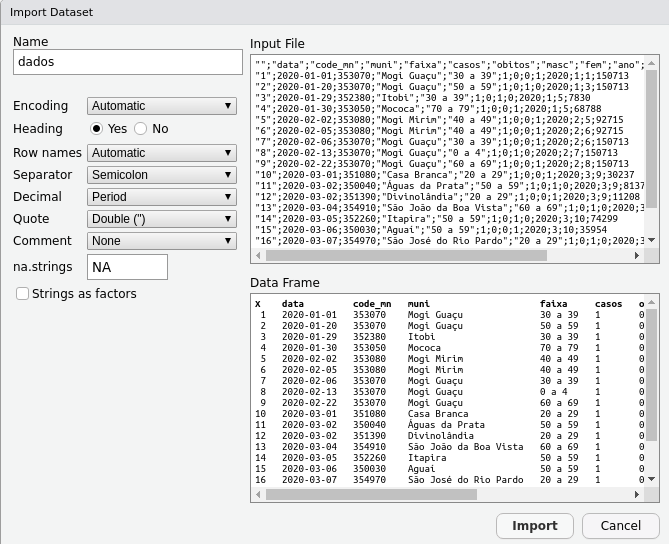
\includegraphics{ilustracoes/import_dataset.png}

\hypertarget{escrita-de-arquivos}{%
\section{Escrita de arquivos}\label{escrita-de-arquivos}}

\hypertarget{utilswrite.csv2}{%
\subsection{utils::write.csv2()}\label{utilswrite.csv2}}

Função para salvar um arquivo de dados que foi trabalhado no R em diferentes formatos, no caso, separado por ponto e vírgula. Um ponto negativo é que essa função, ao salvar o arquivo, cria uma coluna com nomes das linhas (em números), para que isso não ocorra, deve-se utilizar o argumento row.names = FALSE. (\href{https://www.rdocumentation.org/packages/utils/versions/3.6.2/topics/write.table}{documentação}).

\begin{quote}
\textbf{Exemplo}
\end{quote}

\begin{verbatim}
write.csv2(x = iris,                # Dados ativos
           file = 'dados/iris.csv', # Caminho e nome do arquivo
           fileEncoding = "UTF-8", 
           row.names = FALSE)       # Encoding
\end{verbatim}

\begin{quote}
\textbf{Argumentos principais}
\end{quote}

\begin{longtable}[]{@{}
  >{\raggedright\arraybackslash}p{(\columnwidth - 2\tabcolsep) * \real{0.5000}}
  >{\raggedright\arraybackslash}p{(\columnwidth - 2\tabcolsep) * \real{0.5000}}@{}}
\toprule\noalign{}
\begin{minipage}[b]{\linewidth}\raggedright
Argumento
\end{minipage} & \begin{minipage}[b]{\linewidth}\raggedright
Definição
\end{minipage} \\
\midrule\noalign{}
\endhead
\bottomrule\noalign{}
\endlastfoot
x & Objeto a ser escrito, prefereincialmente uma matriz ou data.frame. \\
file & Nome do arquivo criado (pode conter o caminho) utilizando aspas '' ``. \\
append & Logical. Se TRUE os dados serão adicionados à última linha de um arquivo já existente, que deve ter o nome descrito em file, se FALSE qualquer arquivo com o nome descrito será sobrescrito. \\
na & String usada para valores ausentes nos dados. \\
dec & String para definir divisor de decimal, ex. dec = ``.''. \\
col.names & Logical. Indica se os nomes das colunas de x devem ser escritos junto com x, ou um vetor de caracteres dos nomes das colunas a serem escritos. \\
row.names & Logical. Cria coluna com nomes para linhas. \\
fileEncoding & String. Declara a codificação a ser usada para que possam ser recodificados à medida que são gravados. \\
\end{longtable}

\hypertarget{readrwrite_csv2}{%
\subsection{readr::write\_csv2()}\label{readrwrite_csv2}}

É semelhante à função anterior, mas executa a tarefa mais rápido, com a vantagem de não criar uma coluna com nomes das linhas (\href{https://www.rdocumentation.org/packages/readr/versions/1.3.1/topics/write_delim}{documentação}).

\begin{quote}
\textbf{Exemplo}
\end{quote}

\begin{verbatim}
readr::write_csv2(x = iris, file = 'dados/iris.csv')
\end{verbatim}

\begin{quote}
\textbf{Argumentos principais}
\end{quote}

\begin{longtable}[]{@{}
  >{\raggedright\arraybackslash}p{(\columnwidth - 2\tabcolsep) * \real{0.5000}}
  >{\raggedright\arraybackslash}p{(\columnwidth - 2\tabcolsep) * \real{0.5000}}@{}}
\toprule\noalign{}
\begin{minipage}[b]{\linewidth}\raggedright
Argumento
\end{minipage} & \begin{minipage}[b]{\linewidth}\raggedright
Definição
\end{minipage} \\
\midrule\noalign{}
\endhead
\bottomrule\noalign{}
\endlastfoot
x & Um data frame ou tibble a ser escrito. \\
file & Caminho, nome do arquivo e extensão. \\
append & Se FALSE, irá sobrescrever um arquivo existente, caso exista. Se TRUE, será salvo a partir da última linha de um arquivo existente. \\
col\_names & Default TRUE. Primeira linha como nomes das colunas. Se FALSE, nomes das colunas não serão incluídos. \\
\end{longtable}

\hypertarget{writexlwrite_xlsx}{%
\subsection{writexl::write\_xlsx()}\label{writexlwrite_xlsx}}

Grava um dataframe em um arquivo xlsx. Para criar um xlsx com (várias) sheets nomeadas, basta definir x para uma lista nomeada de dataframe (\href{https://www.rdocumentation.org/packages/writexl/versions/1.4.0/topics/write_xlsx}{documentação}).

\begin{quote}
\textbf{Exemplo 1}
\end{quote}

\begin{verbatim}
writexl::write_xlsx(x = iris,
                    path = 'dados/iris.xlsx',
                    col_names = TRUE,      # Primeira linha como nome das colunas
                    format_headers = TRUE) # Inserir nome das colunas
readxl::read_excel('dados/iris.xlsx', n_max = 2)
\end{verbatim}

\begin{quote}
\textbf{Exemplo 2}
\end{quote}

\begin{verbatim}
writexl::write_xlsx(path = "dados/conjuntodadosnativos.xlsx",
           x = list(sheet1=iris, sheet2=cars, sheet3=mtcars))

readxl::read_excel(path = 'dados/conjuntodadosnativos.xlsx',
                   sheet = 3, 
                   n_max = 2)
\end{verbatim}

\begin{quote}
\textbf{Argumentos principais}
\end{quote}

\begin{longtable}[]{@{}
  >{\raggedright\arraybackslash}p{(\columnwidth - 2\tabcolsep) * \real{0.5000}}
  >{\raggedright\arraybackslash}p{(\columnwidth - 2\tabcolsep) * \real{0.5000}}@{}}
\toprule\noalign{}
\begin{minipage}[b]{\linewidth}\raggedright
Argumento
\end{minipage} & \begin{minipage}[b]{\linewidth}\raggedright
Definição
\end{minipage} \\
\midrule\noalign{}
\endhead
\bottomrule\noalign{}
\endlastfoot
x & Data frame ou lista de data frames que serão salvos em planilhas (sheets). \\
path & Nome do arquuivo criado. \\
col\_names & Se TRUE, primera linha traz os nomes das colunas. \\
format\_headers & Inserir nomes das colunas. \\
\end{longtable}

\hypertarget{data.tablefwrite}{%
\subsection{data.table::fwrite()}\label{data.tablefwrite}}

Função para escrever .csv muito mais rápido (por exemplo, 2 segundos versus 1 minuto) e flexível. Máquinas modernas têm mais de uma CPU, então fwrite as usa; em todos os sistemas operacionais, incluindo Linux, Mac e Windows. Output em csv, csv2, tab, etc. (\href{https://www.rdocumentation.org/packages/data.table/versions/1.14.2/topics/fwrite}{documentação}).

\begin{quote}
\textbf{Exemplo}
\end{quote}

\begin{verbatim}
dados <- data.table::fread(file = 'dados/dados.csv', nrows = 20)
data.table::fwrite(x = dados,                     # Objeto a ser escrito
                   file = 'dados/dados20max.csv', # Nome e caminho (arquivo ja exite)
                   append = TRUE,                 # Salva na ultima linha do arquivo ja existente
                   sep = ';',                     # Separados de colunas
                   showProgress = TRUE)           # Mostrar progresso
\end{verbatim}

\begin{quote}
\textbf{Argumentos principais}
\end{quote}

\begin{longtable}[]{@{}
  >{\raggedright\arraybackslash}p{(\columnwidth - 2\tabcolsep) * \real{0.5000}}
  >{\raggedright\arraybackslash}p{(\columnwidth - 2\tabcolsep) * \real{0.5000}}@{}}
\toprule\noalign{}
\begin{minipage}[b]{\linewidth}\raggedright
Argumento
\end{minipage} & \begin{minipage}[b]{\linewidth}\raggedright
Definição
\end{minipage} \\
\midrule\noalign{}
\endhead
\bottomrule\noalign{}
\endlastfoot
x & Objeto a salvar. Deve estar como data.frame ou data.table. \\
file & Nome do arquivo. \\
append & Se TRUE , o arquivo é salvo em acrescimo à última linha de um arquivo existente, sem incluir os nomes das colunas. \\
sep & Separador de colunas. Default é ``,''. \\
na & Um string a ser usada para valores ausentes. O padrão é uma string em branco ``\,``. \\
dec & Separador de decimal, default é ``.''. \\
row.names & Nome das linhas. Usar somente se for data.frame, porque é incompatível com data.table.. \\
col.names & Primeira linha como nomes das colunas. \\
logical01 & Os valores lógicos devem ser escritos como 1 e 0 em vez de ``TRUE'' e ``FALSE''? \\
showProgress & Exibir um medidor de progresso no console. Ignorado quando file == ``\,``. \\
compress & Se compress = ``auto'' e se o arquivo termina em .gz, o formato de saída é gzipado csv. Se compress = ``none'', o formato de saída é sempre csv. Se compress = ``gzip'', o formato é csv compactado com gzip. A saída para o console nunca é compactada com gzip mesmo se compress = ``gzip''. Por padrão, compress = ``auto''. \\
\end{longtable}

\hypertarget{rioexport}{%
\subsection{rio::export()}\label{rioexport}}

Semelhante a outros comandos de escrita de arquivos, o rio::export() permite gravar um data frame nos formatos habituais de texto. Para exportar uma lista de arquivos, usar o rio::export\_list() (\href{https://www.rdocumentation.org/packages/rio/versions/0.5.29/topics/export}{Documentação}).

\begin{quote}
\textbf{Exempĺo}
\end{quote}

\begin{verbatim}
rio::export(x = iris,                  # Objeto que será exportado.
            file = 'dados/iris.xlsx')  # Caminho, nome e extensão.
\end{verbatim}

\begin{quote}
\textbf{Argumentos principais}
\end{quote}

\begin{longtable}[]{@{}
  >{\raggedright\arraybackslash}p{(\columnwidth - 2\tabcolsep) * \real{0.5000}}
  >{\raggedright\arraybackslash}p{(\columnwidth - 2\tabcolsep) * \real{0.5000}}@{}}
\toprule\noalign{}
\begin{minipage}[b]{\linewidth}\raggedright
Argumento
\end{minipage} & \begin{minipage}[b]{\linewidth}\raggedright
Definição
\end{minipage} \\
\midrule\noalign{}
\endhead
\bottomrule\noalign{}
\endlastfoot
x & Matriz ou data frame a ser escrita. Exceções são que x pode ser uma lista de dados se o formato de arquivo de saída for uma pasta de Excel .xlsx. Para exportar uma lista de quadros de dados para vários arquivos, use export\_list em vez disso. \\
file & Nome do arquivo. Deve especificar file e/ou format. \\
format & Sequência de caracteres opcional contendo o formato de arquivo, que pode ser usado para substituir o formato inferido a partir de file ou, em vez de especificar file, um arquivo com o nome do símbolo de x e a extensão de arquivo especificada será criado. Os atalhos incluem: ``,'' ou ``;'' ou '' \\
\end{longtable}

\hypertarget{leitura-de-muxfaltiplos-arquivos}{%
\section{Leitura de múltiplos arquivos}\label{leitura-de-muxfaltiplos-arquivos}}

Particularmente tenho maior interesse na possibilidade de ler e agrupar diversos arquivos, assim, o enfoque desse tópico será sobre a leitura com merge.

\hypertarget{baselapply-e-basereduce}{%
\subsection{base::lapply() e base::Reduce}\label{baselapply-e-basereduce}}

A ideia aqui é fazer a leitura dos arquivos de interesse e juntá-los verticalmente compondo um dataframe final, assim, o método é dividido em três partes:\\
1. Listar os arquivos de interesse presentes no diretório.
2. Fazer leitura múltipla utilizando a função base::lapply e base::read.csv2 (pode ser outra) (\href{https://www.rdocumentation.org/packages/base/versions/3.6.2/topics/lapply}{documentação base::lapply}).
3. Juntar os dataframes com base::Reduce e base::rbind.dataframe (\href{https://www.rdocumentation.org/packages/purrr/versions/0.2.5/topics/reduce}{documentação base::reduce})

\begin{quote}
\textbf{Exemplo 1}
\end{quote}

\begin{verbatim}
setwd('arquivos/')                         # Define a pasta que contém os arquivos
lista <- base::list.files()                # Captura os arquivos na pasta e atribui à uma lista
arquivos <- base::lapply(X = lista,        # Lista com os arquivos a serem lidos
                         FUN = read.csv2)  # Função escolhida para ler
unidos <- base::Reduce(x = arquivos,       # Lista de dataframes
                       f = base::rbind.data.frame)  # Função para empilhar
setwd("~/Documentos/Estudos R/guia_de_bolso") # Volta para diretorio inicial
\end{verbatim}

O base::setwd() é mais importante neste caso por conta da atividade do base::lapply, que não tem um argumento path para definir espaço de trabalho, então o \emph{work directory} tem que ser definido antes.\\
A lista ``arquivos'' também pode ser aplicada à função data.table::rbindlist(), que terá o mesmo efeito da função elaborada no \texttt{reduce}.

\begin{quote}
\textbf{Exemplo 2}
\end{quote}

Aqui a ideia é realizar a leitura, mas filtrando os arquivos somente com os dados de interesse, ao mesmo tempo, para isso, vamos usar a função base::function() (\href{https://www.rdocumentation.org/packages/base/versions/3.6.2/topics/function}{documentação}). Os parâmetros serão passados para essa função e ela será aplicada ao lapply.

\begin{verbatim}
setwd('arquivos2/')

filtro.fun <- function(x){                      # Cria uma função
  data.table::fread(file = x) %>% 
    dplyr::select("Petal.Length",               # Manipulações
                  "Petal.Width", 
                  "Species") %>%
    dplyr::filter(Petal.Length > .5) %>%
    setNames(nm = c("compr","largura","especie"))
}

lista <- list.files()
arquivos <- lapply(X = lista, FUN = filtro.fun)

unidos <- data.table::rbindlist(l = arquivos)  # Mesmo efeito do Reduce

setwd("~/Documentos/Estudos R/guia_de_bolso") # Volta para diretório inicial
\end{verbatim}

\hypertarget{basefor}{%
\subsection{base::for()}\label{basefor}}

A função \texttt{for} permite criar um loop de execução de determinada ação, no caso, o loop do exemplo realizará a leitura de vários arquivos que serão atribuidos à uma lista. Com a lista é possível empilhar em um único data frame. (\href{https://www.rdocumentation.org/packages/base/versions/3.6.2/topics/Control}{documentação}).

\begin{quote}
\textbf{Exemplo}
\end{quote}

\begin{verbatim}
x <- 1                            # Objeto contador
arquivos <- list(rep(NA, 3))      # O objeto que vai receber a leitura individual dos arquivos, deve ser uma lista vazia
lista <- list.files('arquivos2/') # Lista com os arquivos a serem lidos

for (i in lista) {                # Para cada elemento da lista, executar:
  arquivos[[x]] <- read.csv2(file = file.path('arquivos2',i)) %>%  # Cada elemento lido é adicionado a um espaço vazio da lista de arquivos
    filter(Sepal.Length > 5.5)
  x <- x + 1                      # O contador define em que posição o arquivo lido será adicionado à lista de arquivos
}

dados <- data.table::rbindlist(l = arquivos)[1:3,] # os arquivos filtrados foram alocados na lista "arquivos". Agora eles serão empilhados com esta função para definir um banco de dados final com todos os elementos.
\end{verbatim}

\hypertarget{rioimport_list}{%
\subsection{rio::import\_list()}\label{rioimport_list}}

Importa uma lista de data frames de um vetor de nomes ou arquivo multi-objeto (planilha Excel, arquivo .Rdata etc). Realiza a mesma função de lapply() e for(), mas com menos etapas (\href{https://www.rdocumentation.org/packages/rio/versions/0.5.29/topics/import_list}{documentação}).

\begin{quote}
\textbf{Exemplo}
\end{quote}

\begin{verbatim}
setwd('arquivos/')
lista <- list.files()
unidos <- rio::import_list(file = lista,  # Lista com nomes dos arquivos do diretório
                 rbind = TRUE,            # Empilhar linhas 
                 header = TRUE)           # Nomes das colunas
setwd("~/Documentos/Estudos R/guia_de_bolso")
\end{verbatim}

\hypertarget{escrita-de-muxfaltiplos-arquivos}{%
\section{Escrita de múltiplos arquivos}\label{escrita-de-muxfaltiplos-arquivos}}

\hypertarget{rioexport_list}{%
\subsection{rio::export\_list()}\label{rioexport_list}}

Exporta uma lista de data frames. A extensão colocada no nome do arquivo já direciona o formato, porém, pode-se usar o argumento sep = ``;'' ou outro para definir o desejado. Os nomes dos arquivos salvos podem ser declarados por um ou múltiplos verotes, ex. c(``iris1.csv'',``iris2.csv''), ou usar o recurso \texttt{\%s}, ex. \texttt{\%s.csv} que designa o nome do objeto como nome do arquivo que será criado (\texttt{nome\_do\_objeto.csv}) (\href{https://www.rdocumentation.org/packages/rio/versions/0.5.26/topics/export_list}{documentação})

\begin{quote}
\textbf{Exemplo}
\end{quote}

\begin{verbatim}
rio::export_list(x = list(iris1 = iris[1:30,],   # Lista nomeada (iris 1 ...) dos objetos
                          iris2 = iris[60:80,],
                          iris3 = iris[50:70,]),
                 file = 'arquivos2/%s.csv',      # Nome do arquivo contido em %s automaticamente
                 sep=";")     # Separador
\end{verbatim}

\hypertarget{datas}{%
\chapter{Datas}\label{datas}}

\hypertarget{funuxe7uxf5es-buxe1sicas}{%
\section{Funções básicas}\label{funuxe7uxf5es-buxe1sicas}}

Existem muitas funções para se criar variáveis com datas e horas e/ou que podem converter formatos diversos. O formato padrão reconhecido nativamente pelo R é por exemplo \emph{2019-12-10}, portanto, para evitar manipulações, é importante tentar criar e utilizar bancos de dados neste padrão. Abaixo, seguem algumas das funções mais utilizadas:

\begin{longtable}[]{@{}
  >{\raggedright\arraybackslash}p{(\columnwidth - 2\tabcolsep) * \real{0.3750}}
  >{\raggedright\arraybackslash}p{(\columnwidth - 2\tabcolsep) * \real{0.6250}}@{}}
\toprule\noalign{}
\begin{minipage}[b]{\linewidth}\raggedright
Função
\end{minipage} & \begin{minipage}[b]{\linewidth}\raggedright
Utilização
\end{minipage} \\
\midrule\noalign{}
\endhead
\bottomrule\noalign{}
\endlastfoot
base::Sys.Date() & Fornece a data atual a partir da data do sistema \\
base::Sys.time() & Fornece a hora atual a partir da hora do sistema \\
base::date() & Fornece a data no formato: ``Mon Oct 10 17:50:32 2022'' \\
base::as.Date() & Converte um elemento de texto em character, ex: as.Date(``2020-01-31'') \\
base::strftime() & tz = fuso horário \\
base::OlsonNames() & Nomes padronizados de fusos horários \\
base::months() & Extrai o mês no formato string de uma data já formatada, ex: months(as.Date(``2020-05-01'')), resulta ``maio'' \\
base::weekdays() & Retorna o dia da semana que corresponde à data, ex: base::weekdays(as.Date(``2020-05-01'')), resulta ``sexta-feira'' \\
lubridate::ymd() & Converte o texto em data, mantendo o formato \\
lubridate::dmy() & Converte o formato de data brasileiro para o formato padrão do sistema \\
lubridate::dmy\_h() & Retorna a data e horário \\
lubridate::as\_date() & Retorna a data independente do formato de entrada, ex: as\_date(``19/05/2022'', format = ``\%d/\%m/\%Y''), mas se estiver na ordem correta (ex:20200225) ele identifica automaticamente e coloca no formato padrão, ex: as\_date(``20200226'') resulta ``2020-02-26''. Se estiver fora da ordem esperada, ex: as\_date(``01031998'', format = ``\%d\%m\%Y'') \\
lubridate::year(), month(), day() & Extraem o ano, o mês e o dia de uma data, respectivamente \\
lubridate::wday() & Retorna o dia da semana para uma ou mais datas \\
floor\_date(), ceiling\_date() & Arredondam uma data para o intervalo de tempo especificado (por exemplo, semana, mês, ano) \\
data.table::year() & Extrai o ano de uma data, ex: year(``2020-01-31''), resulta 2020 \\
data.table::month() & Extrai o mês de uma data, ex: month(``2020-01-31''), resulta 5 \\
\end{longtable}

\hypertarget{formatar-data-e-hora}{%
\section{Formatar data e hora}\label{formatar-data-e-hora}}

\begin{longtable}[]{@{}
  >{\centering\arraybackslash}p{(\columnwidth - 4\tabcolsep) * \real{0.2308}}
  >{\centering\arraybackslash}p{(\columnwidth - 4\tabcolsep) * \real{0.2308}}
  >{\raggedright\arraybackslash}p{(\columnwidth - 4\tabcolsep) * \real{0.5385}}@{}}
\toprule\noalign{}
\begin{minipage}[b]{\linewidth}\centering
Código
\end{minipage} & \begin{minipage}[b]{\linewidth}\centering
Exemplo
\end{minipage} & \begin{minipage}[b]{\linewidth}\raggedright
Definição
\end{minipage} \\
\midrule\noalign{}
\endhead
\bottomrule\noalign{}
\endlastfoot
\%a & ``ter'' & Nome abreviado do dia da semana. \\
\%A & ``terça-feira'' & Nome completo do dia da semana. \\
\%b & ``out'' & Nome do mês abreviado. \\
\%B & ``outubro'' & Nome completo do mês. \\
\%c & ``ter out 11 00:00:00 2022'' & Data e hora. Equivale a ``\%a \%b \%e \%H:\%M:\%S \%Y''. \\
\%C & ``20'' & Céculo com dois dígitos. \\
\%d & ``11'' & Dia do mês como número decimal (01--31). \\
\%D & ``10/11/22'' & Formato de data como \%m/\%d/\%y. \\
\%e & ``11'' & Dia do mês como número decimal (1--31), com um espaço à esquerda para um número de um dígito. \\
\%F & ``2022-10-11'' & Equivalente a \%Y-\%m-\%d (o formato de data ISO 8601). \\
\%g & ``22'' & Os dois últimos dígitos do ano com base na semana (consulte \%V). \\
\%G & ``2022'' & O ano com base na semana (consulte \%V) como um número decimal. \\
\%h & ``out'' & Equivalente a \%b. \\
\%H & ``12'' & Horas como número decimal (00--23). Como uma exceção especial, strings como `⁠24:00:00⁠' são aceitas para entrada, pois a ISO 8601 permite isso (usado Sys.time() no exemplo). \\
\%I & ``12'' & Horas como número decimal (01--12). \\
\%j & ``284'' & Dia do ano como número decimal (001--366): Para entrada, 366 só é válido em um ano bissexto. \\
\%m & ``10'' & Mês como número decimal (01--12). \\
\%M & ``13'' & Minuto como número decimal (00--59). \\
\%n & ``barra invertina+n'' & Nova linha na saída, espaço em branco arbitrário na entrada. \\
\%p & ``vazio'' & Indicador AM/PM. Usado com \%I e não com \%H. Uma string vazia em algumas localidades \\
\%r & ``12:30:00'' & Para saída, o relógio de 12 horas (usando AM ou PM da localidade): definido apenas em algumas localidades. Equivalente a \%I:\%M:\%S \%p (usado Sys.time() no exemplo). \\
\%R & ``12:30'' & Equivalente a \%H:\%M. \\
\%S & ``52'' & Segundo como inteiro (00--61)(usado Sys.time() no exemplo). \\
\%t & ``barra invertida=t'' & Tab na saída, espaço em branco arbitrário na entrada. \\
\%T & ``12:32:17'' & Equivalente a \%H:\%M:\%S (usado Sys.time() no exemplo). \\
\%u & ``2'' & Dia da semana como um número decimal (1--7, segunda-feira é 1). \\
\%U & ``41'' & Semana do ano como número decimal (00--53) usando domingo como o primeiro dia 1 da semana (e normalmente com o primeiro domingo do ano como dia 1 da semana 1). \\
\%V & ``41'' & Semana do ano como número decimal (01--53) conforme definido na ISO 8601. Se a semana (começando na segunda-feira) contendo 1º de janeiro tiver quatro ou mais dias no novo ano, será considerada a semana 1. Caso contrário, será a última semana do ano anterior e a próxima semana é a semana 1. \\
\%w & ``2'' & Dia da semana como número decimal (0--6, domingo é 0). \\
\%W & ``41'' & Semana do ano como número decimal (00--53) usando segunda-feira como o primeiro dia da semana (e normalmente com a primeira segunda-feira do ano como dia 1 da semana 1). A convenção do Reino Unido. \\
\%x & ``11/10/2022'' & Identifica o padrão da localidade, ``\%y/\%m/\%d'' na entrada. \\
\%X & ``12:42:09'' & Tempo. Específico de localidade na saída, ``\%H:\%M:\%S'' na entrada (usado Sys.time() no exemplo). \\
\%y & ``22'' & Ano sem século (00-99). \\
\%Y & ``2022'' & Ano com século. \\
\%z & ``-300'' & Deslocamento assinado em horas e minutos do UTC, então -0800 está 8 horas atrás do UTC. Valores até +1400 são aceitos. \\
\%Z & ``-03'' & Abreviação de fuso horário como uma cadeia de caracteres (vazio se não estiver disponível)(usado Sys.time() no exemplo). \\
\end{longtable}

\hypertarget{converter-data}{%
\section{Converter data}\label{converter-data}}

\hypertarget{baseas.date}{%
\subsection{base::as.date()}\label{baseas.date}}

É importante que os códigos de definição (m, B, etc) correspondam ao formato do elemento que será convertido, ex: se ``Nov 03 21'', então a conversão precisa de `\%B \%d \%y', porque `B' é o código para mês ``escrito'', não poderia ser `m' que é para mês número. O mesmo se aplica a todos os códigos.

\begin{quote}
Exemplo
\end{quote}

\begin{Shaded}
\begin{Highlighting}[]
\FunctionTok{list}\NormalTok{(base}\SpecialCharTok{::}\FunctionTok{as.Date}\NormalTok{(}\StringTok{\textquotesingle{}03/11/2021\textquotesingle{}}\NormalTok{,  }\AttributeTok{format =} \StringTok{\textquotesingle{}\%d/\%m/\%Y\textquotesingle{}}\NormalTok{),}
\NormalTok{     base}\SpecialCharTok{::}\FunctionTok{as.Date}\NormalTok{(}\StringTok{\textquotesingle{}03{-}Nov{-}2021\textquotesingle{}}\NormalTok{, }\AttributeTok{format =} \StringTok{\textquotesingle{}\%d{-}\%B{-}\%Y\textquotesingle{}}\NormalTok{),}
\NormalTok{     base}\SpecialCharTok{::}\FunctionTok{as.Date}\NormalTok{(}\StringTok{\textquotesingle{}Nov 03 21\textquotesingle{}}\NormalTok{,   }\AttributeTok{format =} \StringTok{\textquotesingle{}\%B \%d \%y\textquotesingle{}}\NormalTok{),}
\NormalTok{     base}\SpecialCharTok{::}\FunctionTok{as.Date}\NormalTok{(}\StringTok{\textquotesingle{}2021/11/03\textquotesingle{}}\NormalTok{,  }\AttributeTok{format =} \StringTok{\textquotesingle{}\%Y/\%m/\%d\textquotesingle{}}\NormalTok{))}
\end{Highlighting}
\end{Shaded}

\begin{verbatim}
## [[1]]
## [1] "2021-11-03"
## 
## [[2]]
## [1] "2021-11-03"
## 
## [[3]]
## [1] "2021-11-03"
## 
## [[4]]
## [1] "2021-11-03"
\end{verbatim}

O vetor pode estar com classe definida como ``character'', logo, se o formato estiver adequado, esta função pode ser utilizada também para converter para data.

\hypertarget{basestrptime}{%
\subsection{base::strptime()}\label{basestrptime}}

Converte o vetor para data e define a ``time zone''.

\begin{quote}
Exemplo
\end{quote}

\begin{Shaded}
\begin{Highlighting}[]
\NormalTok{base}\SpecialCharTok{::}\FunctionTok{strptime}\NormalTok{(}\StringTok{\textquotesingle{}03/11/2021\textquotesingle{}}\NormalTok{, }\AttributeTok{format =} \StringTok{\textquotesingle{}\%d/\%m/\%Y\textquotesingle{}}\NormalTok{)}
\end{Highlighting}
\end{Shaded}

\begin{verbatim}
## [1] "2021-11-03 -03"
\end{verbatim}

\hypertarget{baseformat}{%
\subsection{base::format()}\label{baseformat}}

Converte o formato de um elemento que já definido por classe ``date''.

\begin{quote}
Exemplo
\end{quote}

\begin{Shaded}
\begin{Highlighting}[]
\NormalTok{data }\OtherTok{\textless{}{-}}\NormalTok{ base}\SpecialCharTok{::}\FunctionTok{as.Date}\NormalTok{(}\StringTok{\textquotesingle{}03/11/2021\textquotesingle{}}\NormalTok{, }\AttributeTok{format =} \StringTok{\textquotesingle{}\%d/\%m/\%Y\textquotesingle{}}\NormalTok{)}
\FunctionTok{print}\NormalTok{(data)}
\end{Highlighting}
\end{Shaded}

\begin{verbatim}
## [1] "2021-11-03"
\end{verbatim}

\begin{Shaded}
\begin{Highlighting}[]
\FunctionTok{format}\NormalTok{(data, }\StringTok{\textquotesingle{}\%B{-}\%d{-}\%Y\textquotesingle{}}\NormalTok{)}
\end{Highlighting}
\end{Shaded}

\begin{verbatim}
## [1] "novembro-03-2021"
\end{verbatim}

\hypertarget{operauxe7uxf5es-com-datas}{%
\section{Operações com datas}\label{operauxe7uxf5es-com-datas}}

\hypertarget{somar-uxe0-data}{%
\subsection{Somar à data}\label{somar-uxe0-data}}

Operações como soma ou subtração de datas não são recomendadas, mas podem ser feitas. Qualquer valor numérico adicionado à uma data é compreendido como ``dia''.

\begin{quote}
Exemplo
\end{quote}

\begin{Shaded}
\begin{Highlighting}[]
\NormalTok{data }\OtherTok{\textless{}{-}}\NormalTok{ base}\SpecialCharTok{::}\FunctionTok{as.Date}\NormalTok{(}\StringTok{"2022{-}01{-}01"}\NormalTok{)}
\NormalTok{data}
\end{Highlighting}
\end{Shaded}

\begin{verbatim}
## [1] "2022-01-01"
\end{verbatim}

\begin{Shaded}
\begin{Highlighting}[]
\NormalTok{data }\SpecialCharTok{+} \DecValTok{365}
\end{Highlighting}
\end{Shaded}

\begin{verbatim}
## [1] "2023-01-01"
\end{verbatim}

\begin{Shaded}
\begin{Highlighting}[]
\NormalTok{data }\SpecialCharTok{+} \DecValTok{28}
\end{Highlighting}
\end{Shaded}

\begin{verbatim}
## [1] "2022-01-29"
\end{verbatim}

\hypertarget{diferenuxe7as-entre-datas}{%
\subsection{Diferenças entre datas}\label{diferenuxe7as-entre-datas}}

A função difftime() identifica a diferença entre datas, mas somente nas opções ``units = c(''auto'', ``secs'', ``mins'', ``hours'', ``days'', ``weeks'')``. Para meses ou anos é preciso realizar outros ajustes.

\textbf{Dias e semanas:}

\begin{Shaded}
\begin{Highlighting}[]
\NormalTok{data\_inicio }\OtherTok{\textless{}{-}}\NormalTok{ base}\SpecialCharTok{::}\FunctionTok{as.Date}\NormalTok{(}\StringTok{"2022{-}01{-}01"}\NormalTok{)}
\NormalTok{data\_fim }\OtherTok{\textless{}{-}}\NormalTok{ base}\SpecialCharTok{::}\FunctionTok{as.Date}\NormalTok{(}\StringTok{"2022{-}07{-}13"}\NormalTok{)}

\NormalTok{base}\SpecialCharTok{::}\FunctionTok{difftime}\NormalTok{(}\AttributeTok{time1 =}\NormalTok{ data\_fim, }\AttributeTok{time2 =}\NormalTok{ data\_inicio) }\CommentTok{\#por padrão o resultado é em dias}
\end{Highlighting}
\end{Shaded}

\begin{verbatim}
## Time difference of 193 days
\end{verbatim}

\begin{Shaded}
\begin{Highlighting}[]
\NormalTok{base}\SpecialCharTok{::}\FunctionTok{difftime}\NormalTok{(}\AttributeTok{time1 =}\NormalTok{ data\_fim, }\AttributeTok{time2 =}\NormalTok{ data\_inicio, }\AttributeTok{units =} \StringTok{\textquotesingle{}week\textquotesingle{}}\NormalTok{) }\CommentTok{\#em semanas}
\end{Highlighting}
\end{Shaded}

\begin{verbatim}
## Time difference of 27.57143 weeks
\end{verbatim}

Para obter o resultado numérico (sem a frase), utilizar a função as.numeric().

\textbf{Meses e anos:}

\begin{verbatim}
data_inicio <- base::as.Date('2022-01-01')
data_fim <- base::as.Date('2023-07-01')

meses_diff <- 12 * (lubridate::year(data_fim) - lubridate::year(data_inicio)) + (lubridate::month(data_fim) - lubridate::month(data_inicio))
anos_diff <- meses_diff / 12

meses_diff
# Resultado: 18

anos_diff
# Resultado: 1.5
\end{verbatim}

\textbf{Idade}

\begin{verbatim}
base::as.integer(Sys.Date() - data_nasc)
base::floor(idade_dias / 365.25)
\end{verbatim}

A função base::floor() arredonda um número para baixo, para o inteiro mais próximo. Por exemplo, floor(3.7) resulta em 3 e floor(4.2) resulta em 4. É utilizado para arredondar para o valor inferior mais próximo, que é ideal para se verificar somente os anos de idade completa.

\hypertarget{sequuxeancia-de-datas}{%
\subsection{Sequência de datas}\label{sequuxeancia-de-datas}}

Realiza uma sequência de datas a partir de uma data inicial até alcançar uma data final, que pode ser definida como uma data específicia ou como a data atual ou do sistema.

\textbf{Método 1: função base::seq()}

\begin{verbatim}
data_inicio <- as.Date("2020-01-01")
base::seq(data_inicio,  # data inicial já deve estar com classe "date"
    by="30 days", # incremento à data inicial
    length=3)     # comprimento do vetor, ou seja, quantas vezes o incremento deve ser aplicado
    
# "by = " pode assumir um valor numérico ou texto, mas no contexto de datas deve ser um número acompanhado de texto (2 days, 1 week, 3 months, 6 years; singular ou plural não faz diferença) 
\end{verbatim}

\textbf{Método 2: função base::seq.Date()}

Novamente, a variável de data aqui já deverá estar no formato ``Date''.

\begin{verbatim}
data_inicio <- base::as.Date('2022-01-01')
base::seq.Date(from = data_inicio, to = Sys.Date(), by = "3 months")
\end{verbatim}

\hypertarget{semana-epidemioluxf3gica}{%
\subsection{Semana epidemiológica}\label{semana-epidemioluxf3gica}}

Método mais fácil hoje para obter essa informação é utilizando a função lubridate::epiweek().

\begin{quote}
Exemplo
\end{quote}

\begin{verbatim}
data <- base::seq.Date(from = as.Date("2020-01-01"),
                 to = as.Date("2020-04-30"), by = "day")

lubridate::epiweek(data)
\end{verbatim}

\hypertarget{parts}{%
\chapter{Parts}\label{parts}}

You can add parts to organize one or more book chapters together. Parts can be inserted at the top of an .Rmd file, before the first-level chapter heading in that same file.

Add a numbered part: \texttt{\#\ (PART)\ Act\ one\ \{-\}} (followed by \texttt{\#\ A\ chapter})

Add an unnumbered part: \texttt{\#\ (PART\textbackslash{}*)\ Act\ one\ \{-\}} (followed by \texttt{\#\ A\ chapter})

Add an appendix as a special kind of un-numbered part: \texttt{\#\ (APPENDIX)\ Other\ stuff\ \{-\}} (followed by \texttt{\#\ A\ chapter}). Chapters in an appendix are prepended with letters instead of numbers.

\hypertarget{footnotes-and-citations}{%
\chapter{Footnotes and citations}\label{footnotes-and-citations}}

\hypertarget{footnotes}{%
\section{Footnotes}\label{footnotes}}

Footnotes are put inside the square brackets after a caret \texttt{\^{}{[}{]}}. Like this one \footnote{This is a footnote.}.

\hypertarget{citations}{%
\section{Citations}\label{citations}}

Reference items in your bibliography file(s) using \texttt{@key}.

For example, we are using the \textbf{bookdown} package \citep{R-bookdown} (check out the last code chunk in index.Rmd to see how this citation key was added) in this sample book, which was built on top of R Markdown and \textbf{knitr} \citep{xie2015} (this citation was added manually in an external file book.bib).
Note that the \texttt{.bib} files need to be listed in the index.Rmd with the YAML \texttt{bibliography} key.

The RStudio Visual Markdown Editor can also make it easier to insert citations: \url{https://rstudio.github.io/visual-markdown-editing/\#/citations}

\hypertarget{blocks}{%
\chapter{Blocks}\label{blocks}}

\hypertarget{equations}{%
\section{Equations}\label{equations}}

Here is an equation.

\begin{equation} 
  f\left(k\right) = \binom{n}{k} p^k\left(1-p\right)^{n-k}
  \label{eq:binom}
\end{equation}

You may refer to using \texttt{\textbackslash{}@ref(eq:binom)}, like see Equation \eqref{eq:binom}.

\hypertarget{theorems-and-proofs}{%
\section{Theorems and proofs}\label{theorems-and-proofs}}

Labeled theorems can be referenced in text using \texttt{\textbackslash{}@ref(thm:tri)}, for example, check out this smart theorem \ref{thm:tri}.

\begin{theorem}
\protect\hypertarget{thm:tri}{}\label{thm:tri}For a right triangle, if \(c\) denotes the \emph{length} of the hypotenuse
and \(a\) and \(b\) denote the lengths of the \textbf{other} two sides, we have
\[a^2 + b^2 = c^2\]
\end{theorem}

Read more here \url{https://bookdown.org/yihui/bookdown/markdown-extensions-by-bookdown.html}.

\hypertarget{callout-blocks}{%
\section{Callout blocks}\label{callout-blocks}}

The R Markdown Cookbook provides more help on how to use custom blocks to design your own callouts: \url{https://bookdown.org/yihui/rmarkdown-cookbook/custom-blocks.html}

\hypertarget{sharing-your-book}{%
\chapter{Sharing your book}\label{sharing-your-book}}

\hypertarget{publishing}{%
\section{Publishing}\label{publishing}}

HTML books can be published online, see: \url{https://bookdown.org/yihui/bookdown/publishing.html}

\hypertarget{pages}{%
\section{404 pages}\label{pages}}

By default, users will be directed to a 404 page if they try to access a webpage that cannot be found. If you'd like to customize your 404 page instead of using the default, you may add either a \texttt{\_404.Rmd} or \texttt{\_404.md} file to your project root and use code and/or Markdown syntax.

\hypertarget{metadata-for-sharing}{%
\section{Metadata for sharing}\label{metadata-for-sharing}}

Bookdown HTML books will provide HTML metadata for social sharing on platforms like Twitter, Facebook, and LinkedIn, using information you provide in the \texttt{index.Rmd} YAML. To setup, set the \texttt{url} for your book and the path to your \texttt{cover-image} file. Your book's \texttt{title} and \texttt{description} are also used.

This \texttt{gitbook} uses the same social sharing data across all chapters in your book- all links shared will look the same.

Specify your book's source repository on GitHub using the \texttt{edit} key under the configuration options in the \texttt{\_output.yml} file, which allows users to suggest an edit by linking to a chapter's source file.

Read more about the features of this output format here:

\url{https://pkgs.rstudio.com/bookdown/reference/gitbook.html}

Or use:

\begin{Shaded}
\begin{Highlighting}[]
\NormalTok{?bookdown}\SpecialCharTok{::}\NormalTok{gitbook}
\end{Highlighting}
\end{Shaded}


  \bibliography{book.bib,packages.bib}

\end{document}
